\section{Rotulagem}
\subsection{Rótulo para um ponto}
\hypertarget{tlp}{}
É possível adicionar vários rótulos no mesmo ponto usando esta macro várias vezes.

\begin{NewMacroBox}{tkzLabelPoint}{\oarg{local opções}\parg{point}\var{label}}%
\begin{tabular}{lll}%
argumentos &  exemplo  &                  \\
\midrule
\TAline{point}{\tkzcname{tkzLabelPoint(A)\{\$A\_1\$\}}}{}
opções  & padrão & definição\\
\midrule
\TOline{TikZ opções}{}{cor, posição etc.}
\bottomrule
\end{tabular}

\medskip
Opcionalmente, podemos usar qualquer estilo do \TIKZ, especialmente posicionamento com above, right, etc...
\end{NewMacroBox}

\subsubsection{Exemplo com \tkzcname{tkzLabelPoint}} 
\begin{tkzexample}[latex=7cm,small]  
\begin{tikzpicture}
  \tkzDefPoint(0,0){A}
  \tkzDefPoint(4,0){B}
  \tkzDefPoint(0,3){C}
  \tkzDrawSegments(A,B B,C C,A)
  \tkzDrawPoints(A,B,C)
  \tkzLabelPoint[left,red](A){$A$}
  \tkzLabelPoint[right,blue](B){$B$}
  \tkzLabelPoint[above,purple](C){$C$}  
\end{tikzpicture} 
\end{tkzexample} 

\subsubsection{Rótulo e referência}
 A referência de um ponto é o objeto que permite usar o ponto, o rótulo é o nome do ponto que será exibido.
 
\begin{tkzexample}[latex=6cm,small]
 \begin{tikzpicture}
    \tkzDefPoint(2,0){A} 
    \tkzDrawPoint(A)
    \tkzLabelPoint[above](A){$A_1$}  
  \end{tikzpicture}
 \end{tkzexample}
 
\subsection{Adicionar rótulos aos pontos \tkzcname{tkzLabelPoints}}
É possível colocar vários rótulos rapidamente quando as referências dos pontos são idênticas aos rótulos e quando os rótulos são colocados da mesma maneira em relação aos pontos. Por padrão, \tkzname{below right} é escolhido.
\hypertarget{tlps}{}

\begin{NewMacroBox}{tkzLabelPoints}{\oarg{local opções}\parg{$A_1,A_2,...$}}%
\begin{tabular}{lll}
argumentos &  exemplo & resultado                 \\
\midrule
\TAline{list of points}{\tkzcname{tkzLabelPoints(A,B,C)}}{Exibição de $A$, $B$ e $C$}
\bottomrule
\end{tabular}

\medskip
Esta macro reduz o número de linhas de código, mas não é óbvio que todos os pontos precisem do mesmo posicionamento de rótulo.
\end{NewMacroBox}

\subsubsection{Exemplo com \tkzcname{tkzLabelPoints}}   
\begin{tkzexample}[latex = 6cm,small]  
\begin{tikzpicture}
  \tkzDefPoint(2,3){A}
  \tkzDefShiftPoint[A](30:2){B}
  \tkzDefShiftPoint[A](30:5){C}
  \tkzDrawPoints(A,B,C)
  \tkzLabelPoints(A,B,C) 
\end{tikzpicture} 
\end{tkzexample}
%<--------------------------------------------------------------------------->
%                       tkzAutoLabelPoints
%<--------------------------------------------------------------------------->
\subsection{Posição automática de rótulos \tkzcname{tkzAutoLabelPoints}}
O rótulo de um ponto é colocado em uma direção definida por um centro e um ponto \tkzname{center}. A distância ao ponto é determinada por uma porcentagem da distância entre o centro e o ponto. Esta porcentagem é dada por \tkzname{dist}.
\begin{NewMacroBox}{tkzLabelPoints}{\oarg{local opções}\parg{$A_1,A_2,...$}}%
\begin{tabular}{lll}
argumentos &  exemplo & resultado                 \\
\midrule
\TAline{list of points}{\tkzcname{tkzLabelPoint(A,B,C)}}{Exibição de $A$, $B$ e $C$}
\end{tabular}
\end{NewMacroBox}

\subsubsection{Rótulo para pontos com \tkzcname{tkzAutoLabelPoints}}
Aqui os pontos são posicionados em relação ao centro de gravidade de $A,B,C \text{ e } O$.
\begin{tkzexample}[latex=4cm,small]
\begin{tikzpicture}[scale=1]
 \tkzDefPoint(2,1){O}
 \tkzDefRandPointOn[circle=center O radius 1.5]\tkzGetPoint{A}
 \tkzDefPointBy[rotation=center O angle 100](A)\tkzGetPoint{C}
 \tkzDefPointBy[rotation=center O angle 78](A)\tkzGetPoint{B}
 \tkzDrawCircle(O,A) 
 \tkzDrawPoints(O,A,B,C) 
 \tkzDrawSegments(C,B B,A A,O O,C)
 \tkzDefTriangleCenter[centroid](A,B,C) \tkzGetPoint{O}
 \tkzDrawPoint(tkzPointResult)
 \tkzLabelPoints(O,A,C,B)
\end{tikzpicture}
\end{tkzexample}

\section{Rótulo para um segmento}
\hypertarget{tls}{}
\begin{NewMacroBox}{tkzLabelSegment}{\oarg{local opções}\parg{pt1,pt2}\marg{label}}
Esta macro permite colocar um rótulo ao longo de um segmento ou uma reta. As opções são as do \TIKZ\ por exemplo \tkzname{pos}.

\medskip
\begin{tabular}{lll}%%
argument    & exemplo & definição    \\
\midrule
\TAline{label}{\tkzcname{tkzLabelSegment(A,B)\{$5$\}}}{texto do rótulo}
\TAline{(pt1,pt2)}{(A,B)}{rótulo ao longo de $[AB]$}
\bottomrule
\end{tabular}

\medskip
\begin{tabular}{lll}%
opções  & padrão & definição    \\
\midrule
\TOline{pos}{.5}{posição do rótulo}
\end{tabular}
\end{NewMacroBox}

\subsubsection{Primeiro exemplo}      
\begin{tkzexample}[latex=7 cm,small]
\begin{tikzpicture}
\tkzDefPoint(0,0){A}
\tkzDefPoint(6,0){B}
\tkzDrawSegment(A,B)
\tkzLabelSegment[above,pos=.8](A,B){$a$}
\tkzLabelSegment[below,pos=.2](A,B){$4$}
\end{tikzpicture} 
\end{tkzexample}  

\subsubsection{Exemplo: quadro negro}  
\begin{tkzexample}[latex=6cm,small]
\tikzstyle{background rectangle}=[fill=black]
\begin{tikzpicture}[show background rectangle,scale=.4]
  \tkzDefPoint(0,0){O}
  \tkzDefPoint(1,0){I}
  \tkzDefPoint(10,0){A}
  \tkzDefPointWith[orthogonal normed,K=4](I,A)
   \tkzGetPoint{H}
  \tkzDefMidPoint(O,A) \tkzGetPoint{M}
  \tkzInterLC(I,H)(M,A)\tkzGetPoints{B}{C}   
  \tkzDrawSegments[color=white,line width=1pt](I,H O,A)
  \tkzDrawPoints[color=white](O,I,A,B,M) 
  \tkzMarkRightAngle[color=white,line width=1pt](A,I,B) 
  \tkzDrawArc[color=white,line width=1pt,
              style=dashed](M,A)(O)    
  \tkzLabelSegment[white,right=1ex,pos=.5](I,B){$\sqrt{a}$} 
  \tkzLabelSegment[white,below=1ex,pos=.5](O,I){$1$}   
  \tkzLabelSegment[pos=.6,white,below=1ex](I,A){$a$} 
\end{tikzpicture} 
\end{tkzexample}

\subsubsection{Rótulos e opção: \tkzname{swap}}
\begin{tkzexample}[latex=7cm,small]
\begin{tikzpicture}[rotate=-60]
\tkzSetUpStyle[red,auto]{label style}
\tkzDefPoint(0,1){A}
\tkzDefPoint(2,4){C}
\tkzDefPointWith[orthogonal normed,K=7](C,A)
\tkzGetPoint{B}
\tkzDefSpcTriangle[orthic](A,B,C){N,O,P}
\tkzDefTriangleCenter[circum](A,B,C)
\tkzGetPoint{O}
\tkzDrawPolygon[green!60!black](A,B,C)
\tkzDrawLine[dashed,color=magenta](C,P)
\tkzLabelSegment(B,A){$c$}
\tkzLabelSegment[swap](B,C){$a$}
\tkzLabelSegment[swap](C,A){$b$}
\tkzMarkAngles[size=1,
     color=cyan,mark=|](C,B,A A,C,P)
\tkzMarkAngle[size=0.75,
     color=orange,mark=||](P,C,B)
\tkzMarkAngle[size=0.75,
      color=orange,mark=||](B,A,C)
\tkzMarkRightAngles[german](A,C,B B,P,C)
\tkzAutoLabelPoints[center = O,dist= .1](A,B,C)
 \tkzLabelPoint[below left](P){$P$}
 \end{tikzpicture} 
\end{tkzexample}

\hypertarget{tlss}{}
 \begin{NewMacroBox}{tkzLabelSegments}{\oarg{local opções}\parg{pt1,pt2 pt3,pt4 ...}}%
Os argumentos são uma lista de pares de pontos. Os estilos do \TIKZ\ estão disponíveis para desenho.
\end{NewMacroBox}

\subsubsection{Rótulos para um triângulo isósceles}      
\begin{tkzexample}[latex=6cm,small]
\begin{tikzpicture}[scale=1]
 \tkzDefPoints{0/0/O,2/2/A,4/0/B,6/2/C}
 \tkzDrawSegments(O,A A,B)
 \tkzDrawPoints(O,A,B)
 \tkzDrawLine(O,B)   
 \tkzLabelSegments[color=red,above=4pt](O,A A,B){$a$}
\end{tikzpicture}
\end{tkzexample}  

\section{Adicionar rótulos em uma reta \tkzcname{tkzLabelLine}}%

\begin{NewMacroBox}{tkzLabelLine}{\oarg{local opções}\parg{pt1,pt2}\marg{label}}
\begin{tabular}{lll}%
argumentos &  padrão & definição   \\
\midrule
\TAline{label}{}{\tkzcname{tkzLabelLine(A,B)}\{\$\tkzcname{Delta}\$\}}
\bottomrule
\end{tabular}

\begin{tabular}{lll}%
opções             & padrão & definição   \\
\midrule
\TOline{pos}{.5}{\tkzname{pos} é uma opção para \TIKZ, mas essencial neste caso\dots}
\end{tabular}

Como opção, e além do \tkzname{pos}, você pode usar todos os estilos do \TIKZ, especialmente o posicionamento com \tkzname{above}, \tkzname{right}, \dots
\end{NewMacroBox}

\subsubsection{Exemplo com \tkzcname{tkzLabelLine}}
Uma opção importante é \tkzname{pos}, é a que permite colocar o rótulo ao longo da reta. O valor de \tkzname{pos} pode ser maior que 1 ou negativo.

\begin{tkzexample}[latex=6cm,small]
\begin{tikzpicture}
   \tkzDefPoints{0/0/A,3/0/B,1/1/C}
   \tkzDefLine[perpendicular=through C,K=-1](A,B)
   \tkzGetPoint{c}
   \tkzDrawLines(A,B C,c)
   \tkzLabelLine[pos=1.25,blue,right](C,c){$(\delta)$} 
   \tkzLabelLine[pos=-0.25,red,left](C,c){again $(\delta)$} 
\end{tikzpicture}
\end{tkzexample}

\subsection{Rótulo em um ângulo: \tkzcname{tkzLabelAngle}}

\begin{NewMacroBox}{tkzLabelAngle}{\oarg{local opções}\parg{A,O,B}}%
Há apenas uma opção, dist (com ou sem unidade), que pode ser substituída pela opção pos do TikZ (sem unidade para esta última). Por padrão, o valor está em centímetros.

\begin{tabular}{lll}%
  \toprule
opções             & padrão & definição                        \\
\midrule
\TOline{pos}{1}{ ou dist, controla a distância do vértice ao rótulo.}
\bottomrule
\end{tabular}

\medskip
É possível mover o rótulo com todas as opções do TikZ: rotate, shift, below, etc.
\end{NewMacroBox}

\subsubsection{Exemplo autor js bibra stackexchange} 
\begin{tkzexample}[latex=7cm,small]
\begin{tikzpicture}[scale=.75]
  \tkzDefPoint(0,0){C}
  \tkzDefPoint(20:9){B}
  \tkzDefPoint(80:5){A}
  \tkzDefPointsBy[projection=onto B--C](A){a}
  \tkzDrawPolygon[thick,fill=yellow!15](A,B,C)
  \tkzDrawSegment[dashed, red](A,a)   
  \tkzDrawSegment[style=red, dashed, 
  dim={$10$,15pt,midway,font=\scriptsize,
   rotate=90}](A,a) 
  \tkzMarkAngle(B,C,A)
  \tkzMarkRightAngle(A,a,C)    
  \tkzMarkRightAngle(C,A,B)
  \tkzFillAngle[fill=blue!20, opacity=0.5](B,C,A)
  \tkzFillAngle[fill=red!20, opacity=0.5](A,B,C)
  \tkzLabelAngle[pos=1.25](A,B,C){$\beta$}
  \tkzLabelAngle[pos=1.25](B,C,A){$\alpha$}
  \tkzMarkAngle(A,B,C)
  \tkzDrawPoints(A,B,C)
  \tkzLabelPoints(B,C)
  \tkzLabelPoints[above](A)
\end{tikzpicture}
\end{tkzexample}

\subsubsection{With \tkzname{pos}} 
\begin{tkzexample}[latex=7cm,small]
\begin{tikzpicture}[scale=.75]
  \tkzDefPoints{0/0/O,5/0/A,3/4/B}
  \tkzMarkAngle[size = 4,mark = ||,
      arc=ll,color = red](A,O,B)%     
  \tkzDrawLines(O,A O,B)
  \tkzDrawPoints(O,A,B)
  \tkzLabelAngle[pos=2,draw,circle,
      fill=blue!10](A,O,B){$\alpha$} 
\end{tikzpicture}
\end{tkzexample}

\subsubsection{\tkzname{pos} and \tkzcname{tkzLabelAngles}} 
\begin{tkzexample}[latex=7cm,small]
\begin{tikzpicture}[rotate=30]
  \tkzDefPoint(2,1){S} 
  \tkzDefPoint(7,3){T}
  \tkzDefPointBy[rotation=center S angle 60](T)
  \tkzGetPoint{P} 
  \tkzDefLine[bisector,normed](T,S,P)
  \tkzGetPoint{s}
  \tkzDrawPoints(S,T,P)   
  \tkzDrawPolygon[color=blue](S,T,P) 
  \tkzDrawLine[dashed,color=blue,add=0 and 3](S,s)  
  \tkzLabelPoint[above right](P){$P$}
  \tkzLabelPoints(S,T)
  \tkzMarkAngle[size = 1.8,mark = |,arc=ll,
                    color = blue](T,S,P)
  \tkzMarkAngle[size = 2.1,mark = |,arc=l,
                    color = blue](T,S,s)
  \tkzMarkAngle[size = 2.3,mark = |,arc=l,
                    color = blue](s,S,P)  
 \tkzLabelAngle[pos = 1.5](T,S,P){$60^{\circ}$}%    
 \tkzLabelAngles[pos = 2.7](T,S,s s,S,P){%
                            $30^{\circ}$}%   
\end{tikzpicture}
\end{tkzexample}


\begin{NewMacroBox}{tkzLabelAngles}{\oarg{local opções}\parg{A,O,B}\parg{A',O',B'}etc.}%
Com opções comuns, há uma macro para múltiplos ângulos.
\end{NewMacroBox}

Finalmente resta poder dar um rótulo para designar um círculo e se várias possibilidades são oferecidas, veremos aqui \tkzcname{tkzLabelCircle}.

\subsection{Dando um rótulo a um círculo}
\begin{NewMacroBox}{tkzLabelCircle}{\oarg{tikz opções}\parg{O,A}\parg{angle}\marg{label}}%
\begin{tabular}{lll}%
opções             & padrão & definição                         \\
\midrule
\TOline{tikz opções} {}{círculo $O$ centro passando por $A$}
\bottomrule
\end{tabular}

\medskip
\emph{ Podemos usar os estilos do \TIKZ. O rótulo é criado e, portanto, \code{passado} entre chaves.}
\end{NewMacroBox} 

\subsubsection{Exemplo}  
\begin{tkzexample}[latex=5cm,small] 
\begin{tikzpicture}
 \tkzDefPoint(0,0){O} \tkzDefPoint(2,0){N}
 \tkzDefPointBy[rotation=center O angle 50](N) 
     \tkzGetPoint{M}
 \tkzDefPointBy[rotation=center O angle -20](N) 
      \tkzGetPoint{P}
 \tkzDefPointBy[rotation=center O angle 125](N) 
      \tkzGetPoint{P'}
 \tkzLabelCircle[above=4pt](O,N)(120){$\mathcal{C}$}
 \tkzDrawCircle(O,M) 
 \tkzFillCircle[color=blue!10,opacity=.4](O,M) 
 \tkzLabelCircle[draw,
       text width=2cm,text centered,left=24pt](O,M)(-120)%
          {The circle\\ $\mathcal{C}$}  
 \tkzDrawPoints(M,P)\tkzLabelPoints[right](M,P)   
\end{tikzpicture}      
\end{tkzexample} 

\section{Rótulo para um arco}
\hypertarget{tls}{}
\begin{NewMacroBox}{tkzLabelArc}{\oarg{local opções}\parg{pt1,pt2,pt3}\marg{label}}
Esta macro permite colocar um rótulo ao longo de um arco. As opções são as do \TIKZ\ por exemplo \tkzname{pos}.

\medskip
\begin{tabular}{lll}%%
argument    & exemplo & definição    \\
\midrule
\TAline{label}{\tkzcname{tkzLabelArc(A,B)\{$5$\}}}{texto do rótulo}
\TAline{(pt1,pt2,pt3)}{(O,A,B)}{rótulo ao longo do arco $\widearc{AB}$}
\bottomrule
\end{tabular}

\medskip
\begin{tabular}{lll}%
opções  & padrão & definição    \\
\midrule
\TOline{pos}{.5}{posição do rótulo}
\end{tabular}
\end{NewMacroBox}

\subsubsection{Rótulo em arco}      
\begin{tkzexample}[latex=7 cm,small]
\begin{tikzpicture}
\tkzDefPoint(0,0){O}
\pgfmathsetmacro\r{2}
\tkzDefPoint(30:\r){A}
\tkzDefPoint(85:\r){B}
\tkzDrawCircle(O,A)
\tkzDrawPoints(B,A,O)
\tkzLabelArc[right=2pt](O,A,B){$\widearc{AB}$}
\tkzLabelPoints(A,B,O)
\end{tikzpicture}
\end{tkzexample}

\endinput